% !TeX spellcheck = en_GB
\documentclass[9pt,twocolumn,twoside,lineno]{pnas-new}
% Use the lineno option to display guide line numbers if required.

\templatetype{pnasresearcharticle}

\title{Public Perceptions on the Coal Debate on Twitter: Reactions to a Corporate Decision-Making Policy Process}

% Use letters for affiliations, numbers to show equal authorship (if applicable) and to indicate the corresponding author
\author[a,b,1]{Yuan Ting Lee}

\affil[a]{Hertie School, Friedrichstr. 180, Berlin 10117, Germany}
\affil[b]{Mercator Research Institute on Global Commons and Climate Change, Torgauer Str. 12 - 15, Berlin 10829, Germany}

% Please give the surname of the lead author for the running footer
\leadauthor{Lee} 

% Please include corresponding author, author contribution and author declaration information
\authorcontributions{}
\authordeclaration{}
\equalauthors{}
\correspondingauthor{\textsuperscript{1}To whom correspondence should be addressed. E-mail: y.lee@mpp.hertie-school.org}

% Keywords are not mandatory, but authors are strongly encouraged to provide them. If provided, please include two to five keywords, separated by the pipe symbol, e.g:
%\keywords{Keyword 1 $|$ Keyword 2 $|$ Keyword 3 $|$ ...} 

\begin{abstract}
Abstract goes here
\end{abstract}

\dates{This manuscript was compiled on \today}

\begin{document}

\maketitle
\thispagestyle{firststyle}
\ifthenelse{\boolean{shortarticle}}{\ifthenelse{\boolean{singlecolumn}}{\abscontentformatted}{\abscontent}}{}

\dropcap{M}ulti-stakeholder commissions have been an important instrument for incorporating external expertise into political decision-making in Germany. It can be seen as an element of ``negotiation democracy”, whereby the experts in the commission decide on an outcome via deliberations and negotiations. Depending on the policy field, representatives of business, science, the social partners, churches, associations and societies can be appointed and thus accelerate the later public discussion. \cite{Siefken2016}

The Coal Commission, formally known as the Commission on Growth, Structural Change and Employment, is such an example of expert commissions. It was set up by the German government under the Federal Ministry for Economy and Energy (BMWi), and was tasked with developing an overarching approach to managing the coal phase-out’s technical, legal, economic and social impacts.

\textbf{Criticisms have emerged about the process of the coal commission, namely that ....}

The process of the German coal commission thus presents a unique situation for analysis: is there a relationship between the seemingly ``corporatist” process of such an expert commission and public opinion, as represented on social media, on the topic? Here, tweets from Twitter are used to represent public opinion on social media, in part due to their high granularity which allows for observations on swiftly changing temporal patterns on topic salience.



\section*{Related Work}

Twitter has been used as a medium to analyse human sentiment through the analysis of variations in the frequency of specific words used by individuals. In \cite{Dodds2011}, Dodds et. al. develop a tool for measuring expressed happiness via positive and negative sentiment in large-scale text corpora. Since its development, the tool, named the ``hedonometer”, has been implemented in studies involving the happiness of cities and states, the happiness of the English language as a whole, the relationship between individuals' happiness and that of those they connect with, and as a method of unsolicited public opinion polling on climate change. \cite{Cody2015} % cite cite !

\section*{Task}
This project aims to identify whether there was an effect on public opinion on the German coal exit throughout the entire decision-making process of the coal commission. To do so, significant events throughout the coal commission process have to be identified and a measure for public opinion has to be designed. Here, public opinion is abstracted from sentiment analysis of tweets made throughout the timeline of the coal commission's lifetime using polarity weighting. 

In addition, in order to understand the public reaction to the deliberative process of the coal commission, it is necessary to understand the broader coal debate on Twitter and how Twitter users on the platform engage in the coal debate -- both on the topic in comparison to other debates, as well as with fellow users on the same topic. 

\section*{Data}
The data used in this project was collected via a two-part process, using two python packages: \texttt{twint} to download the tweets based on specific queries, and \texttt{tweepy} to populate the tweets with extended tweet information. %be more specific and clear here

% insert figure on data collection

The selection process for choosing tweets to analyse stems from the research question at hand, which is to understand the greater coal debate in Germany on Twitter. The final collection of tweets thus include two sets of tweets collected using two different search strategies. The first search strategy includes terms that directly relate to the coal exit in Germany - \{Kohlekommission, Kohleausstieg, Kohlefrei\}.\footnote{Translation: Coal commission, Coal exit, Coal free}

The other set of tweets is obtained from a general search for tweets on coal ("Kohle"), which are then filtered by the inclusion of relevant hashtags in the text of the tweets. These relevant hashtags are obtained by conducting a frequency analysis of all hashtags that appear in "Kohle" tweets, and manually selecting the top hashtags that are related to coal in climate policy. These hashtags are:  \{\#Klimaschutz, \#Hambacherforst, \#Hambibleibt, \#endcoal, \#fridaysforfuture, \#klimawandel, \#klima, and \#endegelaende\}.\footnote{Translation: Climate policy, Hambach Forest, Stay Hambach (forest), Climate Change, Climate, End of the Site} 

The two collections are then combined and duplicates are removed, and the final set is then filtered for tweets in German, which can be obtained as a result from querying the Twitter API. 

In addition to the above set, another set of tweets was collected to use as a baseline for comparison. This set includes the search terms of \{Klima, Erderwärmung, globale Erärmung, Treibhauseffekt\}\footnote{Translation: Climate, Earth warming,Global warming, Greenhouse effect}.

\begin{figure} 
	\begin{center}
		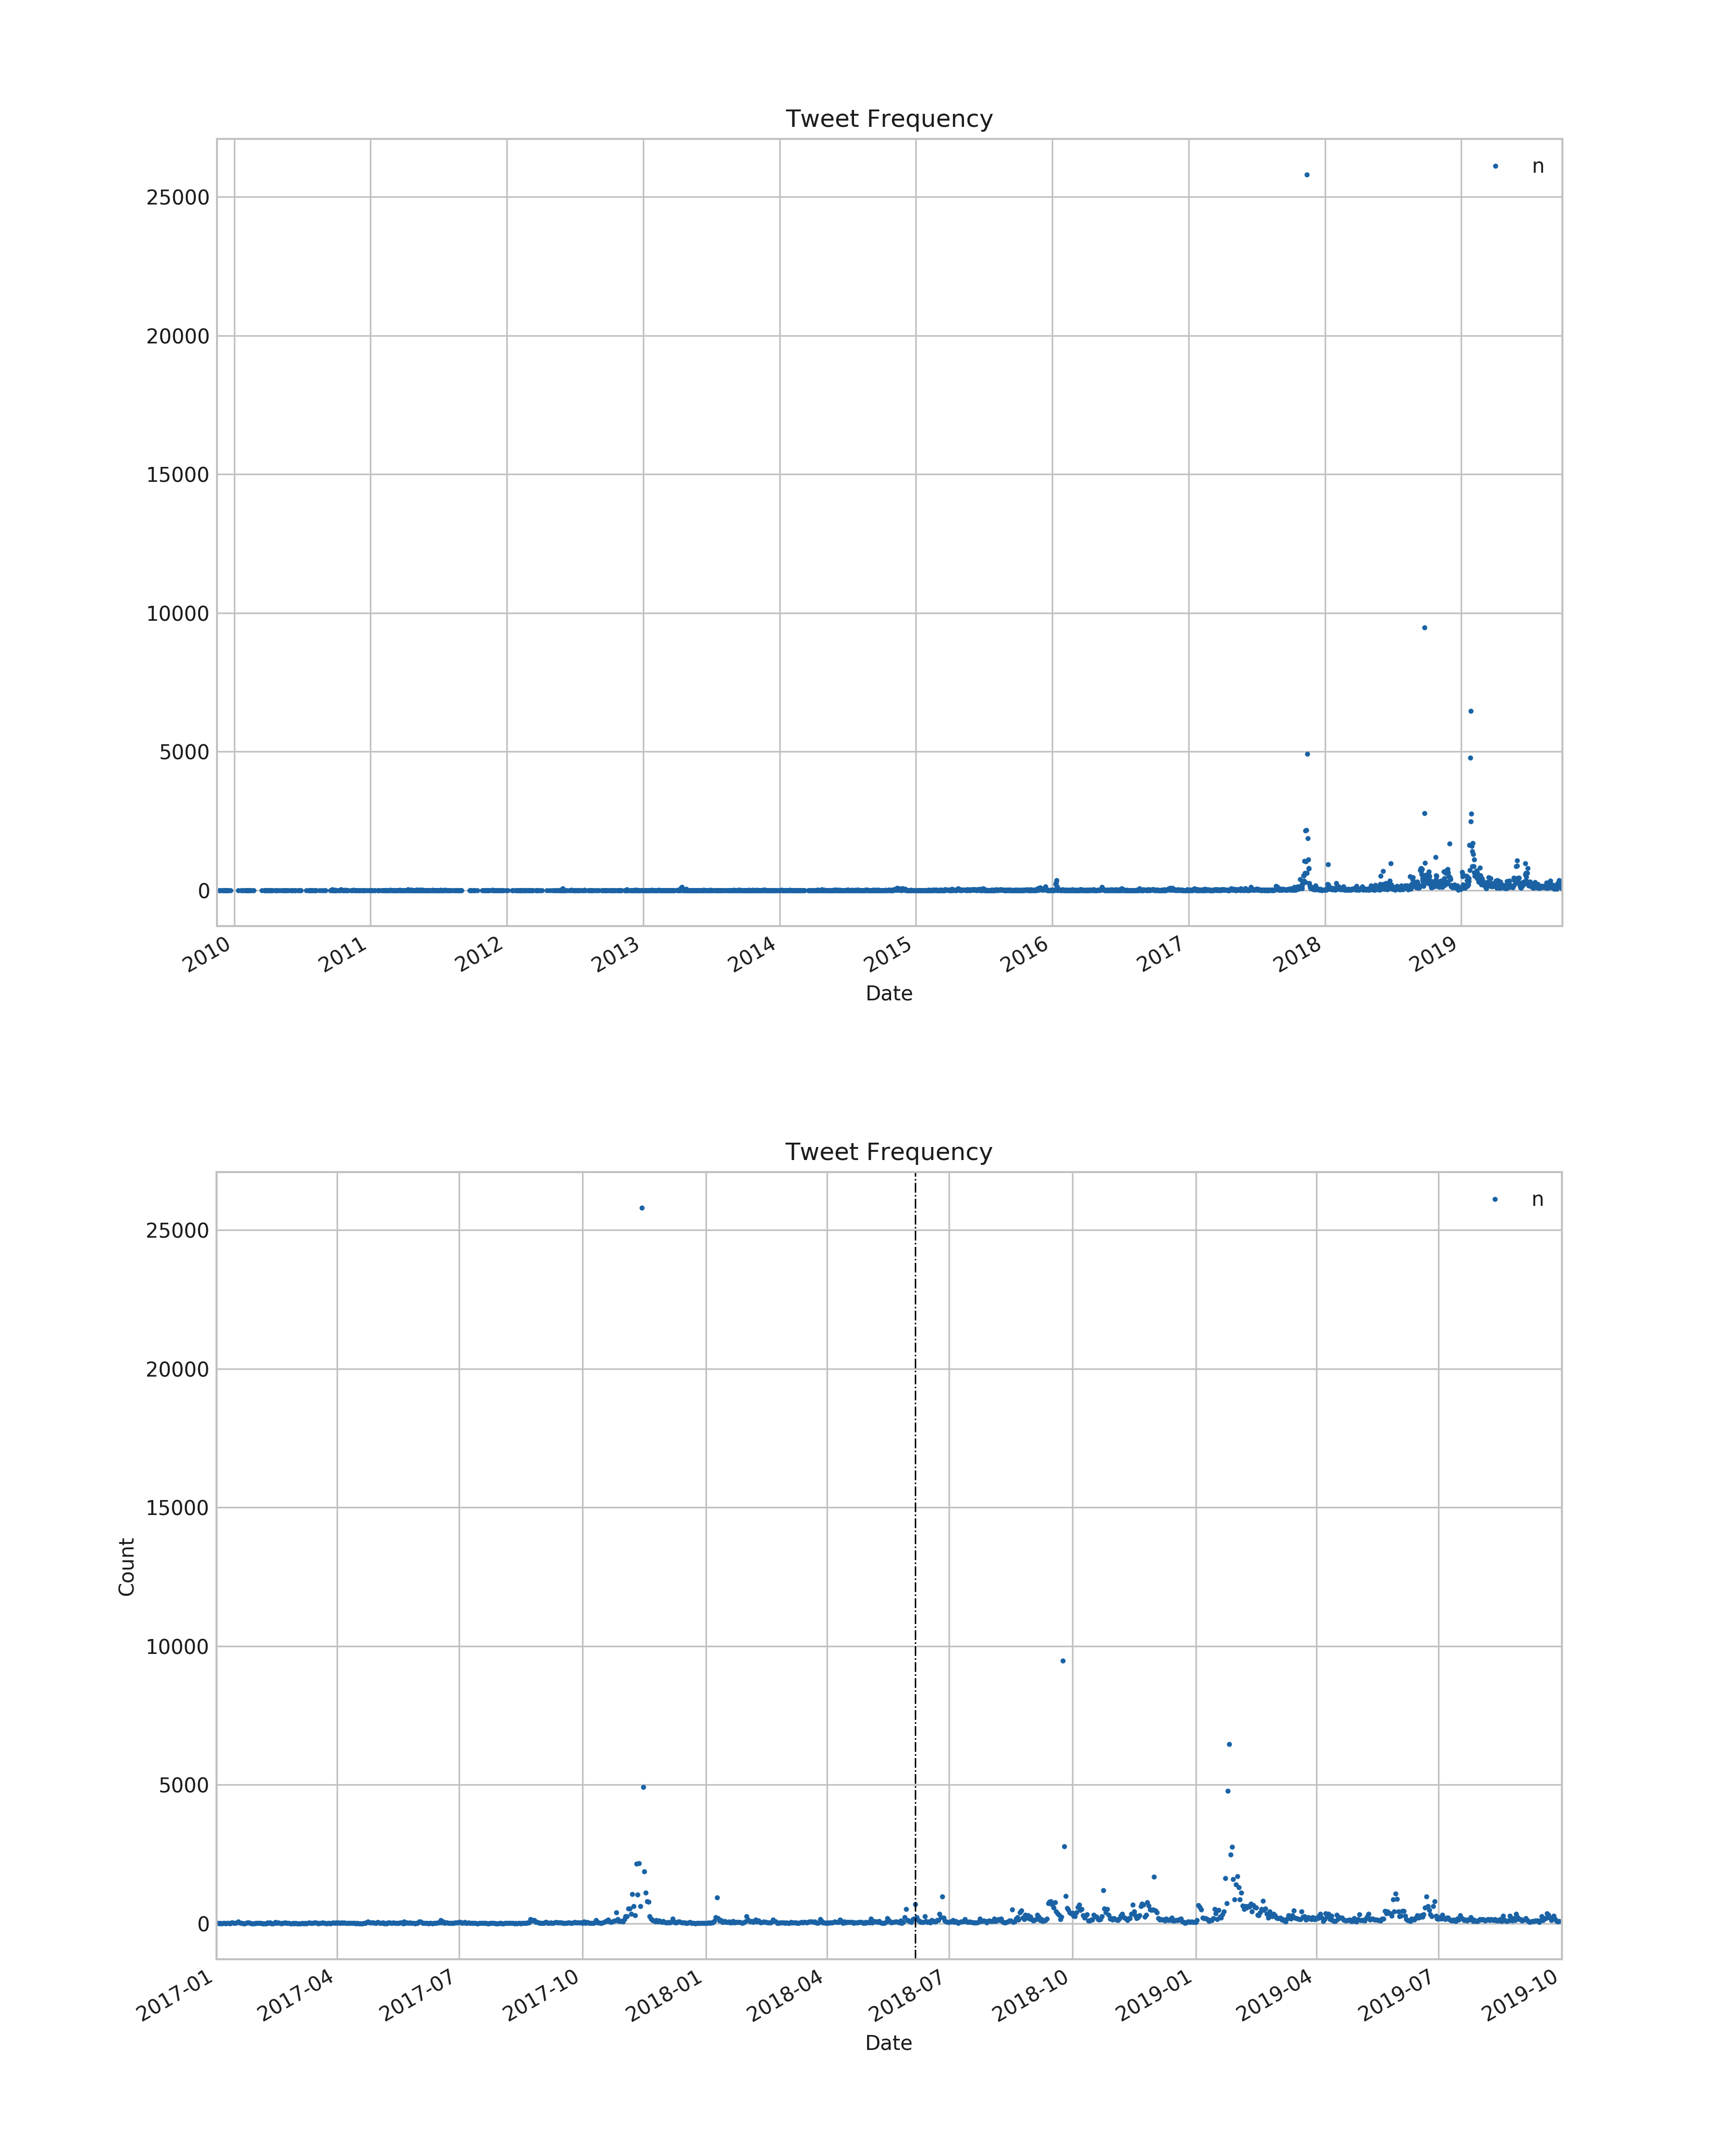
\includegraphics[width=\linewidth]{figures/tweet_frequency_combine}
	\end{center}
	\caption{Daily frequency of tweets in combined dataset, over entire collection period and over coal commission process}
	\label{fig:tweet_frequency}
\end{figure}

\section*{Proposed Method}
\subsection*{Sentiment Analysis}
% Explanation of sentiment analysis 

Sentiment analysis refers to the use of natural language processing and text analysis to systematically identify and extract affective states and subjective information in text. % cite?

The dictionary used is SentiWS, a publicly available German-language resource for sentiment analysis. \cite{REMUS10.490} Entries in the SentiWS dictionary set have four components: the word, its Part of Speech (POS) tag, a polarity weight, and inflections associated with the word, as seen in Fig. \ref{fig:sentiws_example}. The semantic orientations of the words are obtained from three different sources with manual revision. 

The weights of word entries in SentiWS are retrieved using a method known as \emph{Pointwise Mutual Information} (PMI), first suggested in \cite{church-hanks-1990-word}. This approach was successfully re-used for sentiment analysis -- the determination of the semantic orientation and the strength of adjectives -- in \cite{Turney2002} and \cite{Turney2003}, where semantic orientation is inferred from \emph{semantic association}. The semantic orientation \(SO\) of a given word \(w\) is calculated from the strength of its association \(A\) with a manually-selected set of positive seed words \(P\) minus the strength of its association with a set of negative seed words \(N\) (cf. Equation \ref{eq:semantic_orientation}). 

\begin{equation}
\label{eq:semantic_orientation}
\text{SO-A}(w) = \sum_{p \in P}A(w,p) - \sum_{n \in N}A(w,n)
\end{equation}

The word \(w\) is classified as having a positive semantic orientation when SO-A(\(w\)) is positive and a negative semantic orientation SO-A(\(w\)) is negative. The absolute value of SO-A(\(w\)) can be considered the strength of its semantic orientation. 

Parallel to the paradigms in \cite{Turney2003}, SentiWS uses a set of German seed words, from which the semantic associations \(A(w,p)\) and \(A(w,n)\) are calculated using PMI (Equation \ref{eq:pmi}): 

\begin{equation}
\label{eq:pmi}
\text{PMI}(w_1,w_2) = \log_2\left(\frac{P(w_1 \& w_2)}{P(w_1) \cdot P(w_2)}\right)
\end{equation}
where \(P(w)\) is the probability that \(w\) occurs and \(P(w_1 \& w_2)\) is the probability that \(w_1\) and \(w_2\) co-occur. The probabilities were estimated using frequencies and co-occurrence statistics on an internal German-language corpus by the creators of SentiWS consisting of approximately 100 Million sentences. The final weights are then scaled to the interval of [-1;1] and rounded to 4 decimal places with +1.0 being absolutely positive and −1.0 being absolutely negative.

\begin{figure} 
	\begin{center}
		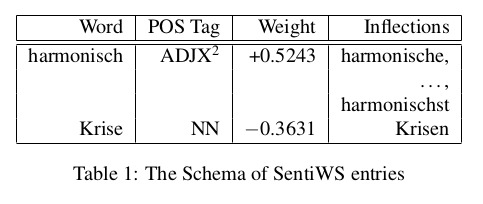
\includegraphics[width=\linewidth]{figures/sentiws_example}
	\end{center}
	\caption{Schema of SentiWS entries}
	\label{fig:sentiws_example}
\end{figure}

To obtain the sentiment score of a tweet, denoted by \(s_{tweet}\), the following formula is used: 

\begin{equation}
\label{eq:word_score}
s_{tweet} = \frac{\sum_{i=1}^{n} s_i f_i}{\sum_{i=1}^{n} f_i}
\end{equation} 
where \(s_i\) is the polarity weighting score of a word given in SentiWS, and \(f_i\) is the frequency of occurrence of the word in the tweet. 



\section*{Results}

\begin{figure} 
	\begin{center}
		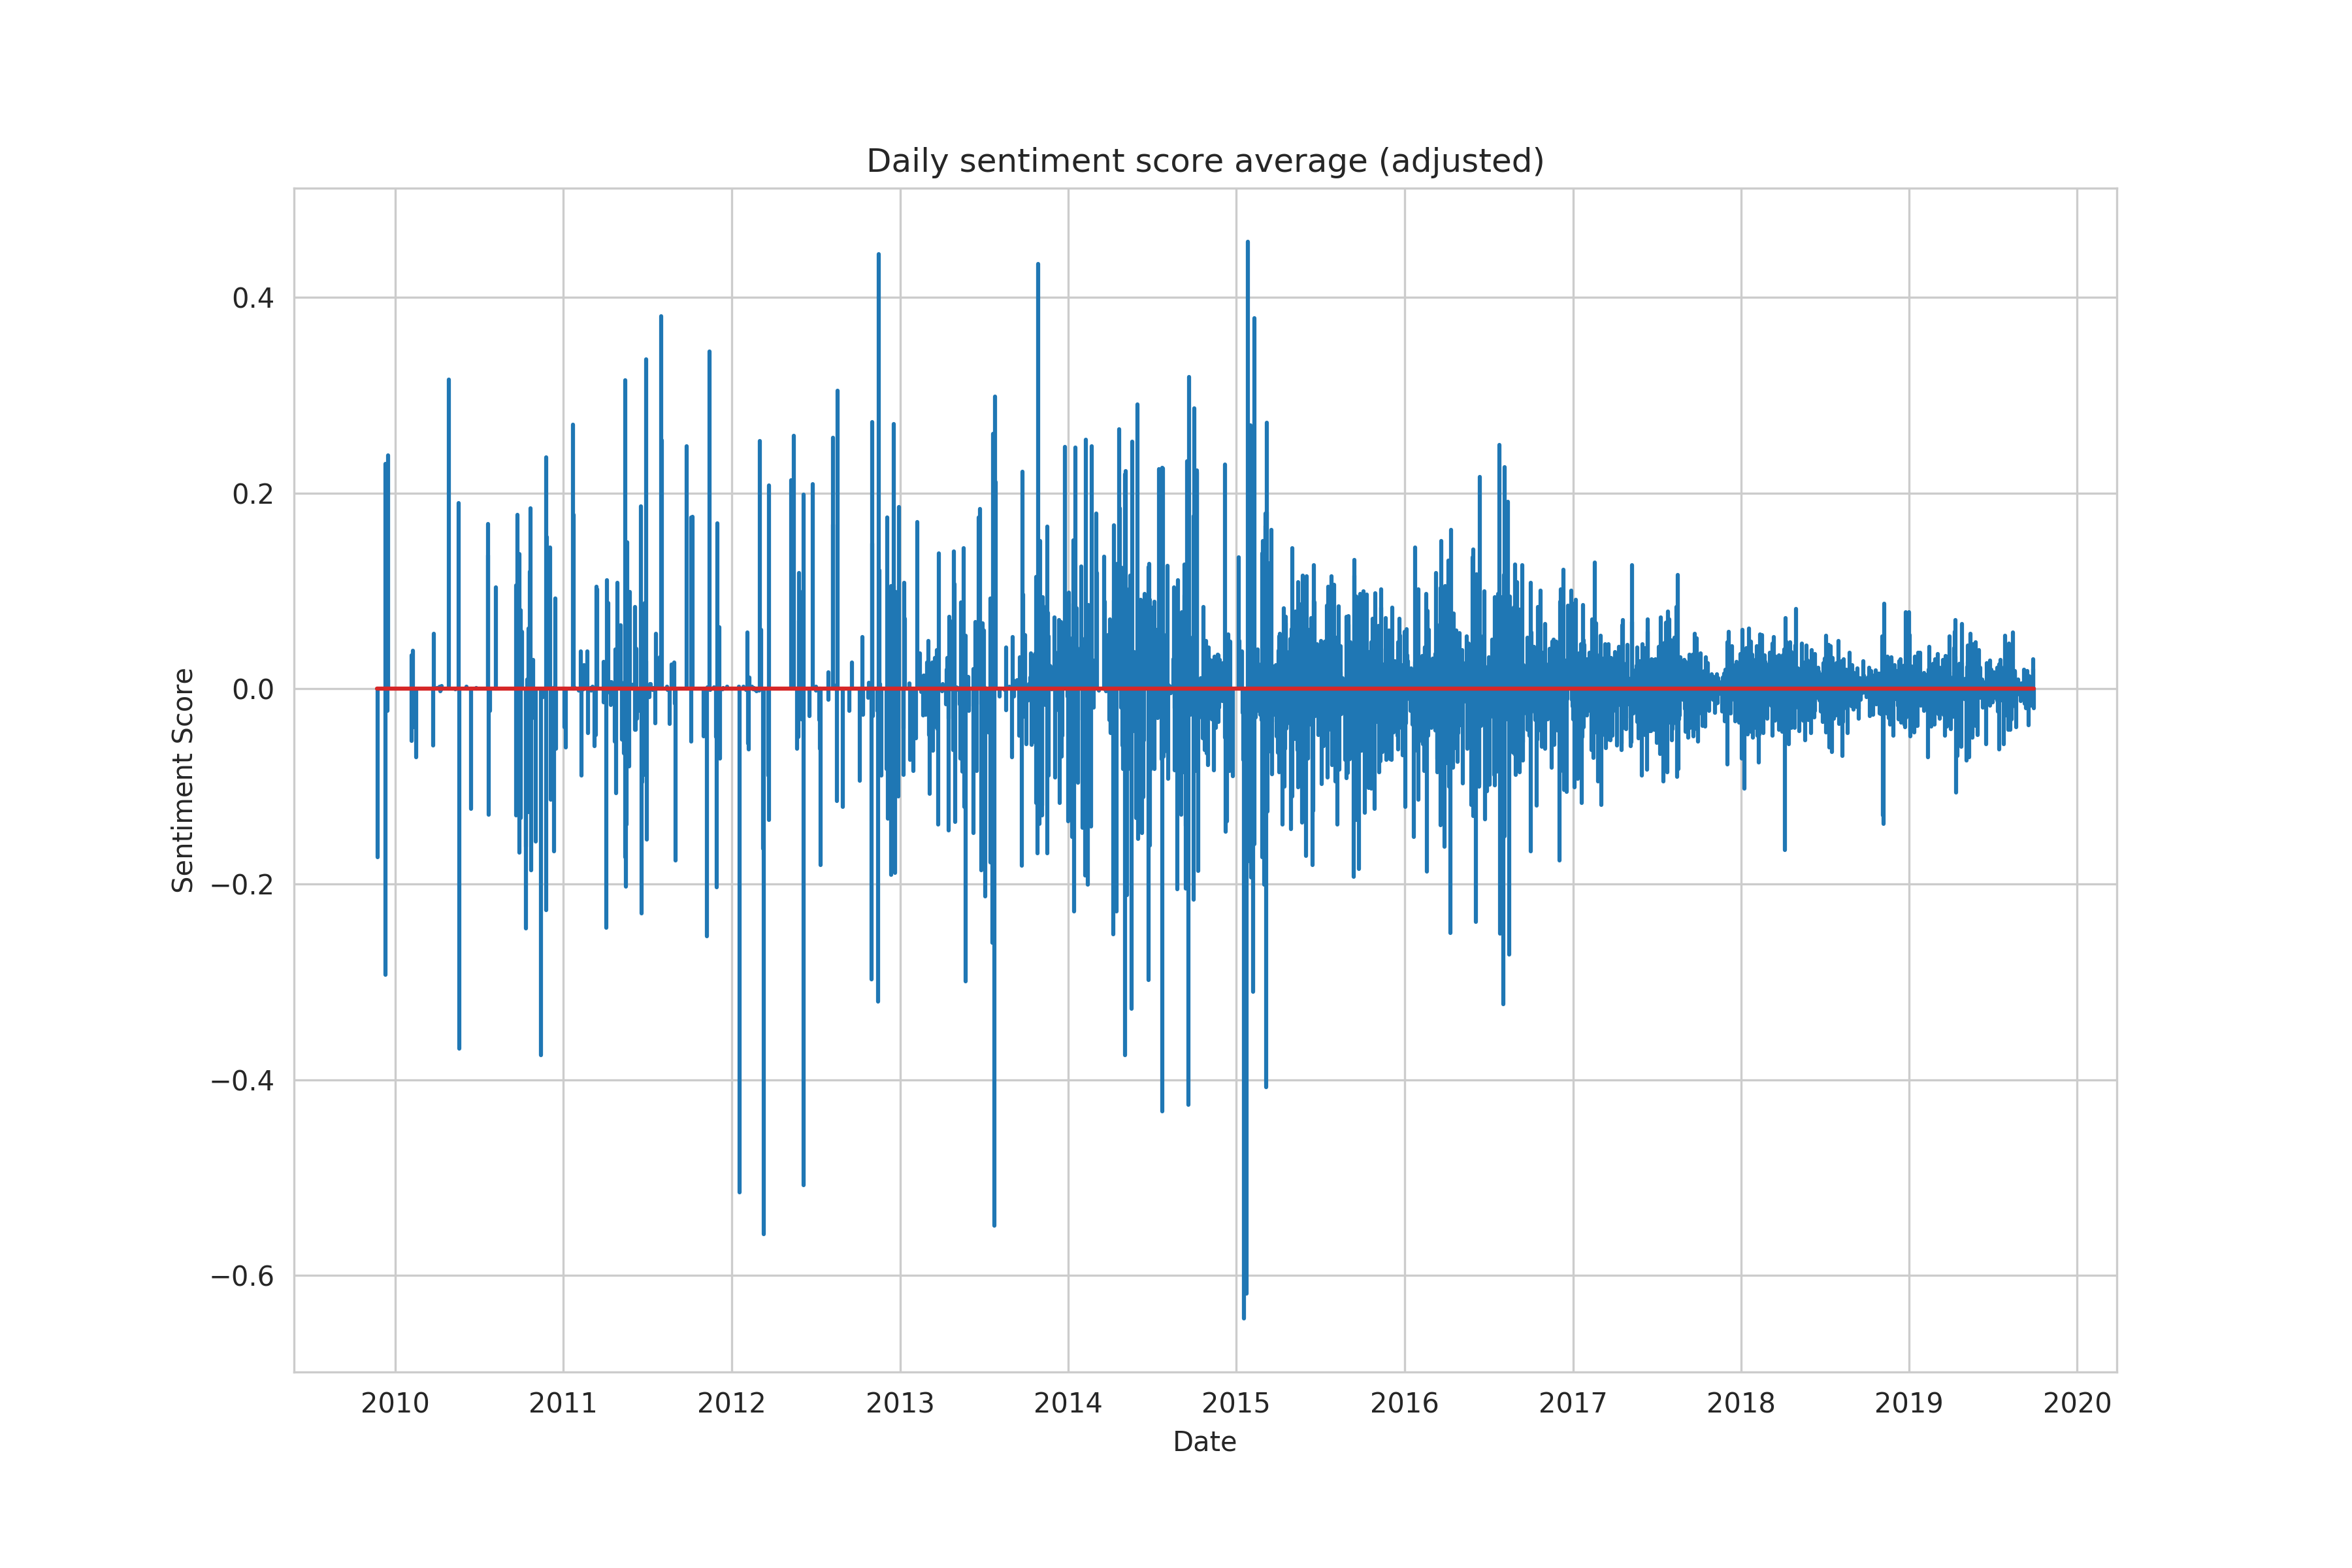
\includegraphics[width=\linewidth]{figures/dailyavgsenti_adjusted}
	\end{center}
	\caption{Daily average sentiment score of tweets, adjusted for 3 day moving average}
	\label{fig:tweet_score_adjusted}
\end{figure}

\begin{figure}
	\begin{center}
		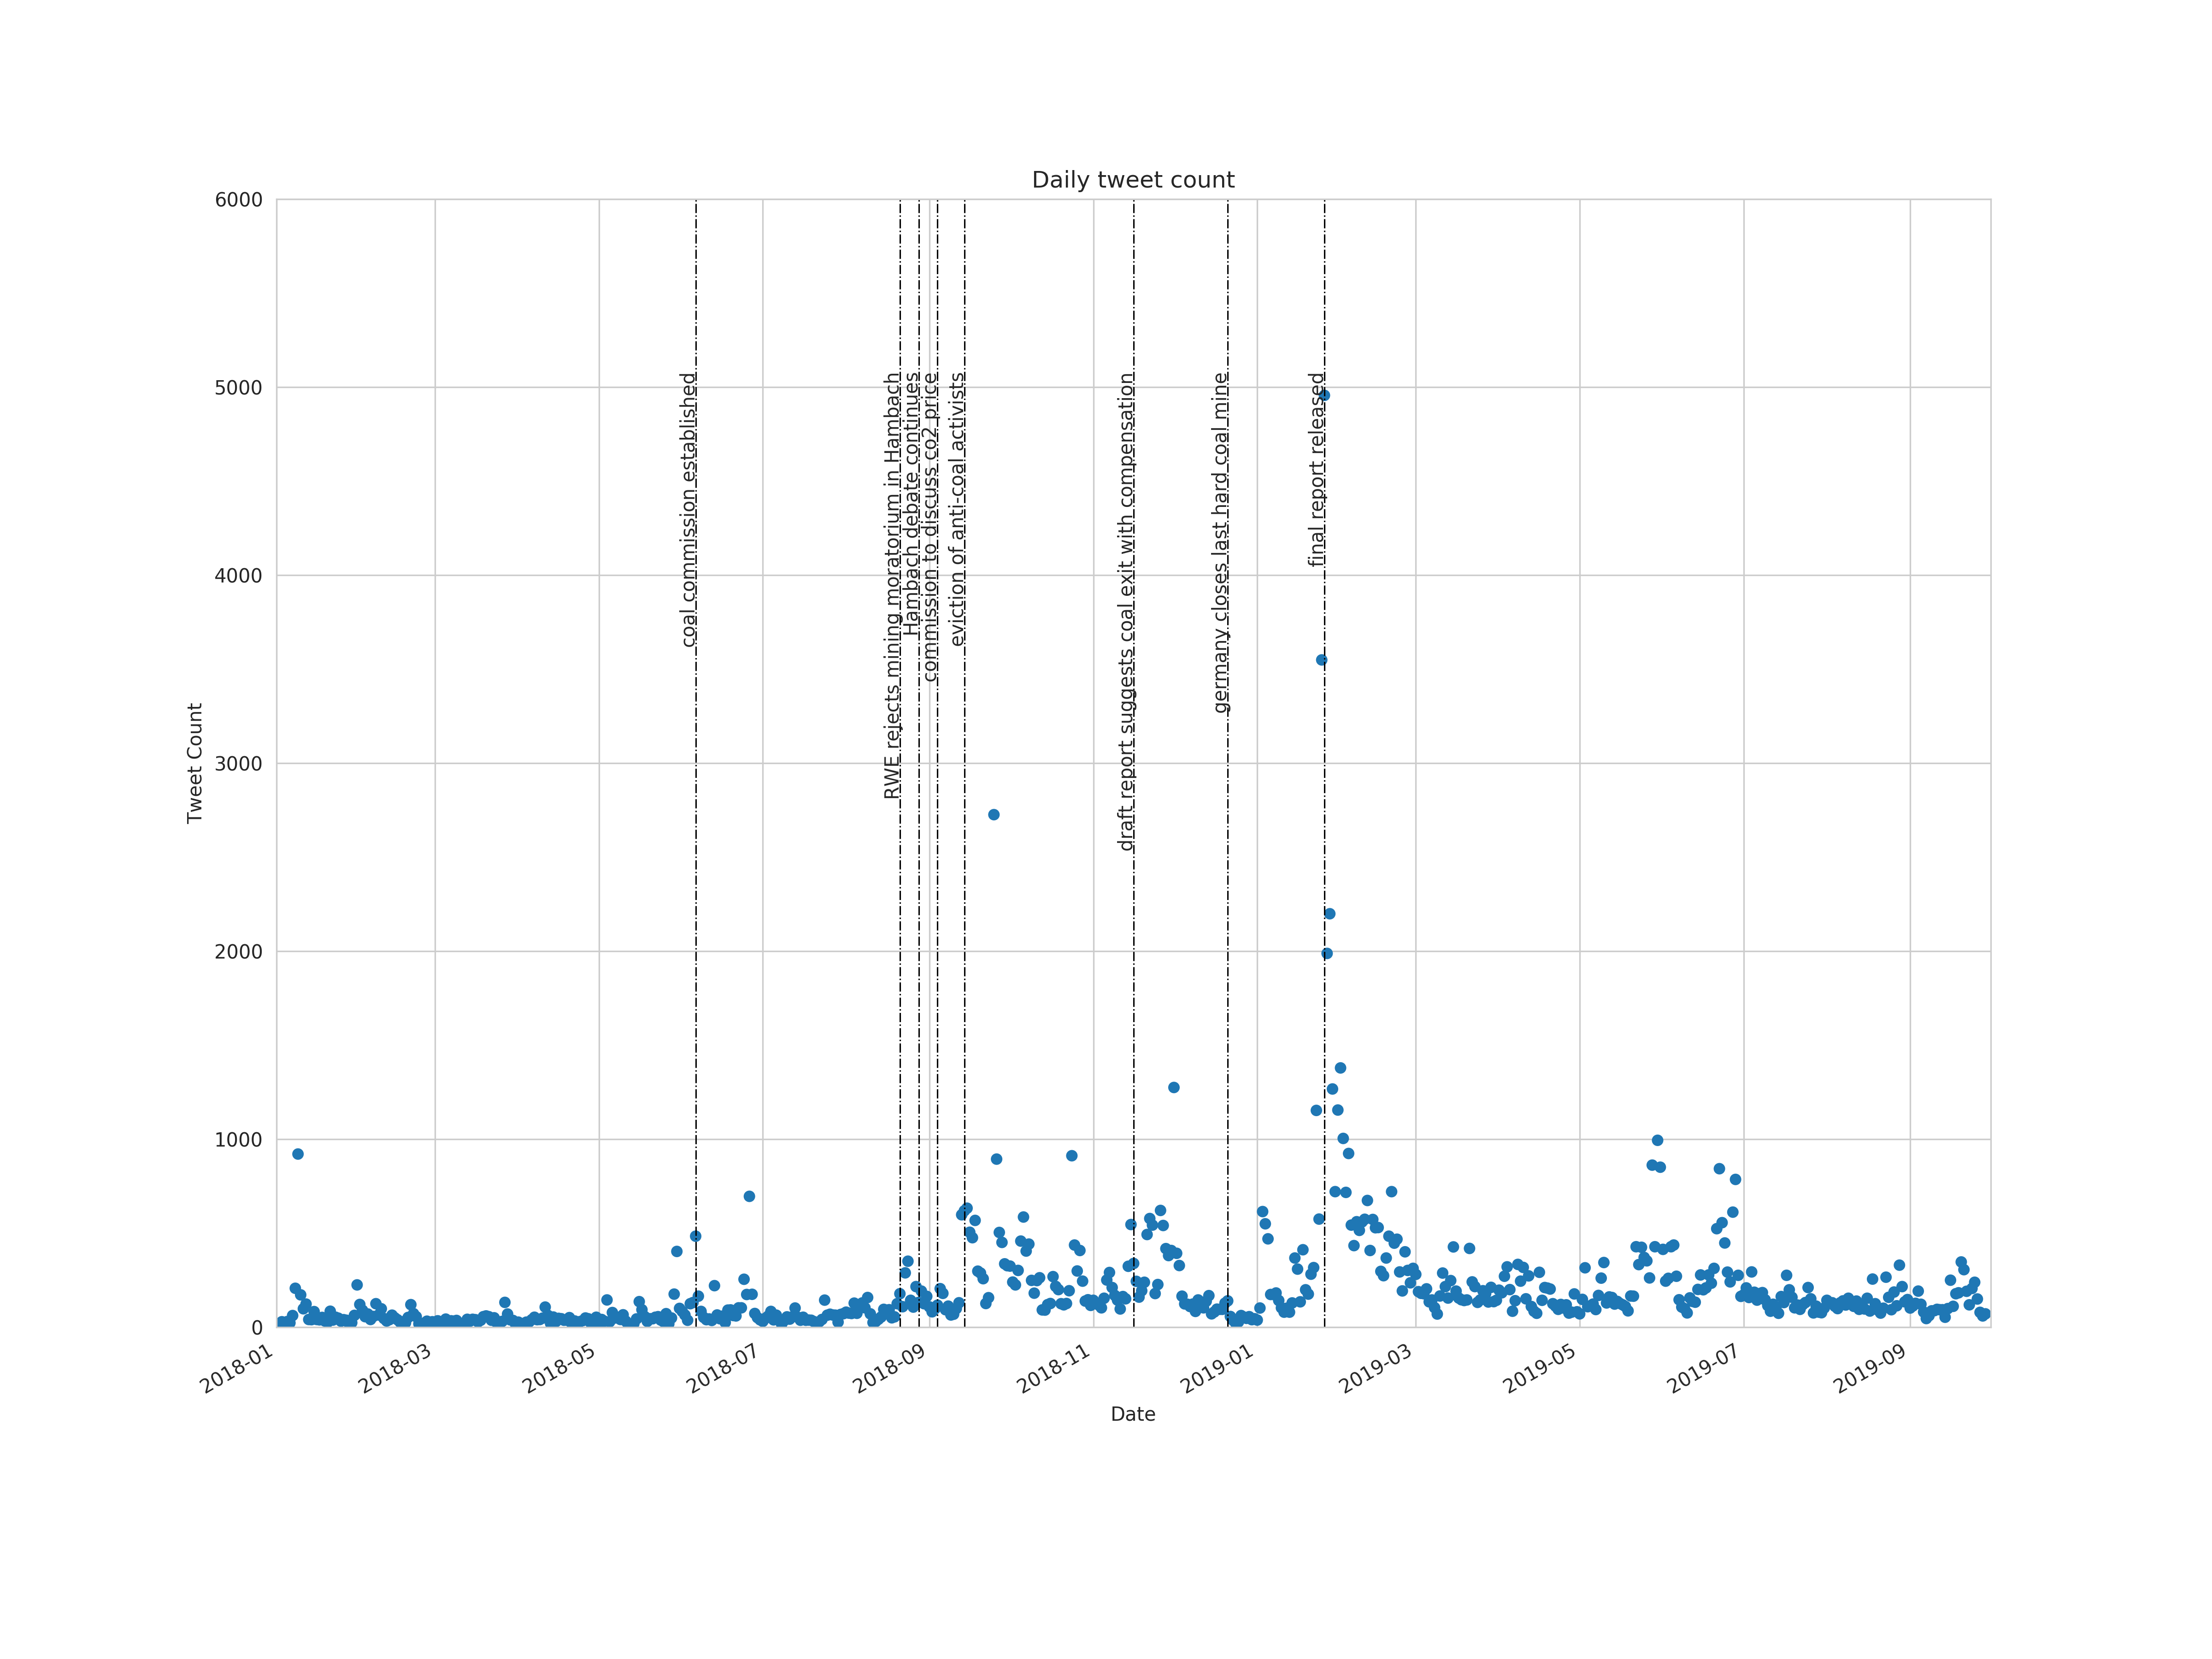
\includegraphics[width=\linewidth]{figures/tweet_count_event_timeline}
	\end{center}
	\caption{Daily count of tweets throughout coal commission process against events throughout coal commission process}
	\label{fig:tweet_count_event_timeline}
\end{figure}

Fig. \ref{fig:tweet_score_adjusted} shows the daily average tweet scores, corrected for with a 3 day moving average. At a glance, the variation in sentiment scores decrease over time. This could signify the reaching of a consensus over time as opinions tend to converge, thus leading to less extreme sentiments being displayed. 

\subsubsection*{Event Analysis} 
Significant events from the coal commission process were taken from Clean Energy Wire's report on the events following the coal commission. \cite{Amelang2019} In Fig. \ref{fig:tweet_score_event_timeline}, the date of significant events are overlaid on the same plot as the daily average sentiment score of tweets. 
 
\begin{figure} 
	\begin{center}
		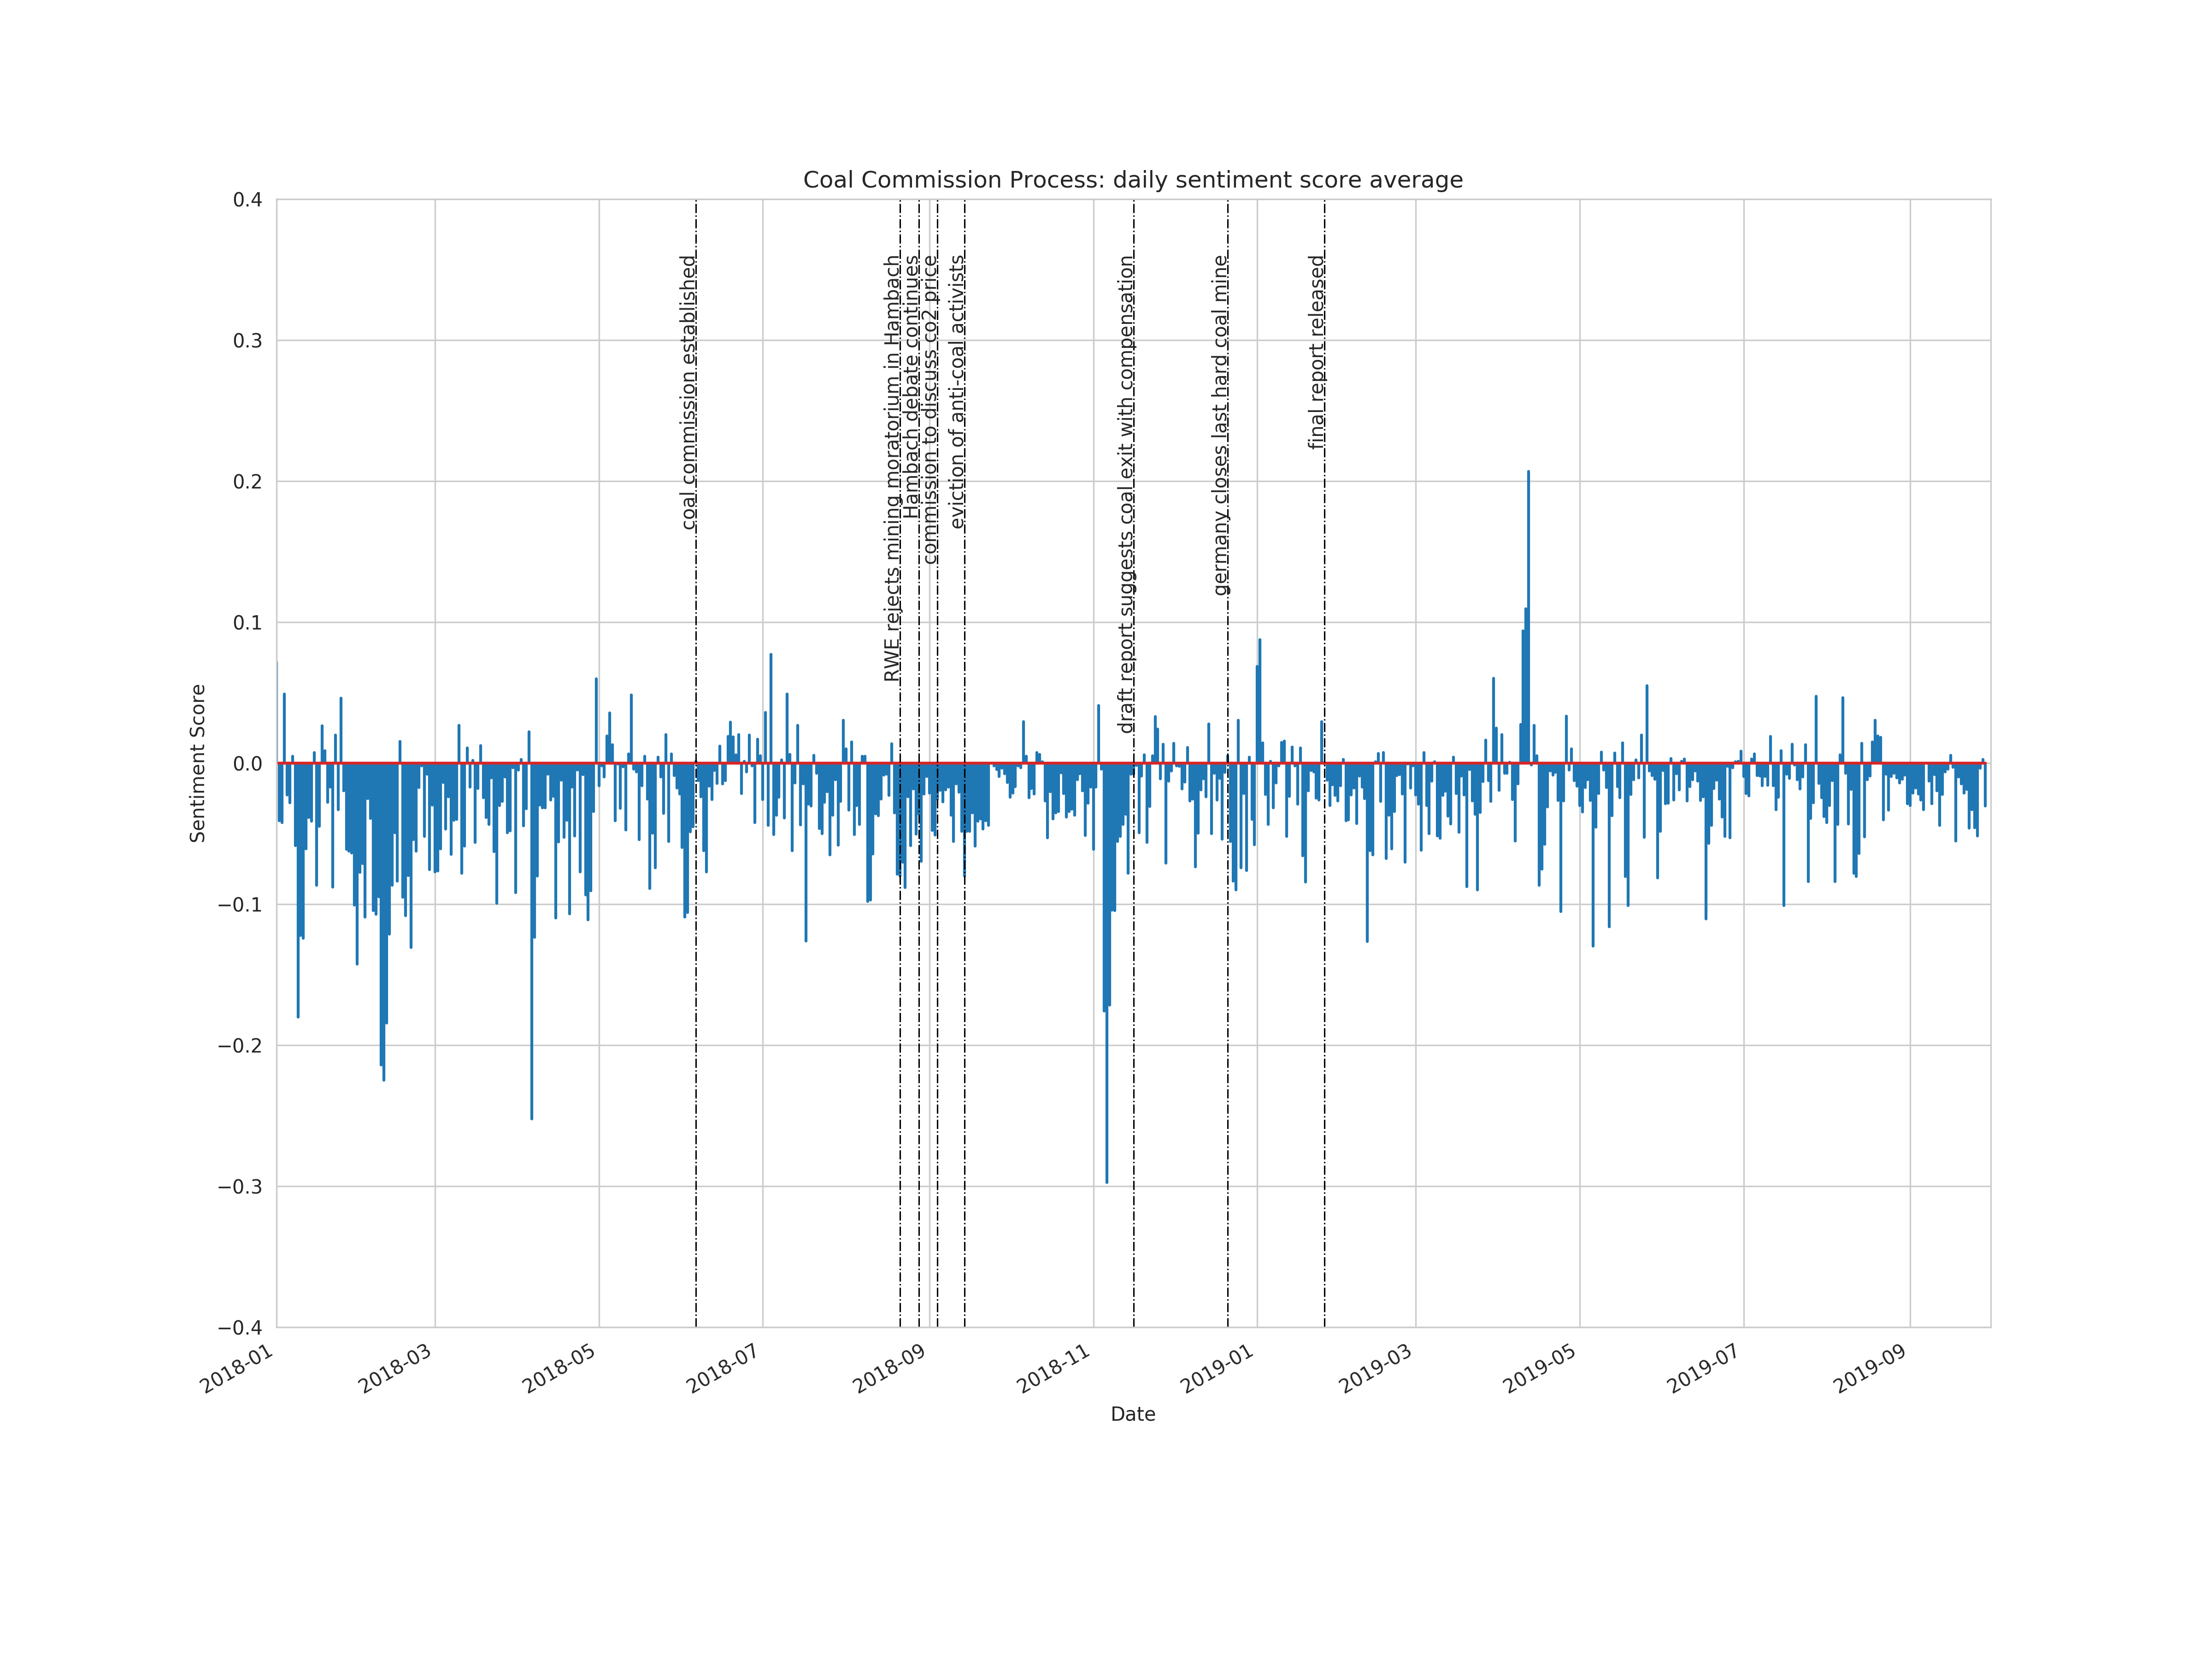
\includegraphics[width=\linewidth]{figures/tweet_score_event_timeline}
	\end{center}
	\caption{Daily average sentiment score of tweets against events throughout coal commission process}
	\label{fig:tweet_score_event_timeline}
\end{figure}

A further look at specific events in \ref{fig:tweet_count_event_timeline} show that there is an uptick in the frequency of tweets when significant events take place. In particular, the day with the most number of tweets in the dataset was on the 26th of January 2019, which was when the coal commission released its final report with recommendations on how to manage the coal phase-out in Germany. 

\subsubsection*{Word Shift}
In order to understand how the debate evolved over time, the tweet dataset used so far is split into two categories by date -- before the establishment of the coal commission and after. The tweets that were made after the coal commission was established are then analysed in comparison to the tweets that were made before the coal commission's establishment. This presents an opportunity to look at how the debate changed over time, whether the focus of the debate had changed after the coal commission began its decision-making process, and how public sentiment changed over the course of the same process. 

In order to assess whether the focus of the debate had changed, topic modelling was performed on the two tweet sets, using the non-negative matrix factorisation (NMF) method with 5 topics. Fig. \ref{fig:topics_before} and \ref{fig:topics_after} show the top 10 words from the topics inferred from the two different sets of tweets. 

\begin{figure} 
	\begin{center}
		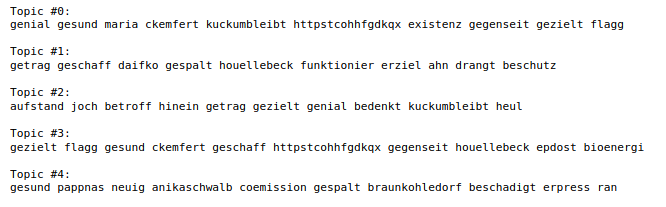
\includegraphics[width=\linewidth]{figures/topics_before}
	\end{center}
	\caption{Topics from tweets made before coal commission establishment}
	\label{fig:topics_before}
\end{figure}
 
\begin{figure} 
	\begin{center}
		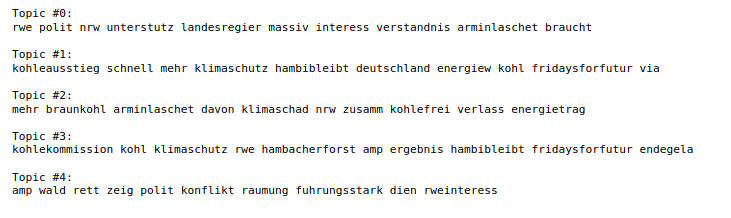
\includegraphics[width=\linewidth]{figures/topics_after}
	\end{center}
	\caption{Topics from tweets made after coal commission establishment}
	\label{fig:topics_after}
\end{figure}

To look at how the language and sentiment changed over time, a method known as ``word valence shift graphs", first used in \cite{Dodds2011}, is employed. To do so, words are ranked by their absolute contributions to the change in average sentiment of one group relative to another. 

% work for this not yet done
In addition, in order to understand the debate on the German coal exit on Twitter, it is necessary to compare it to other debates on Twitter. Here, the climate debate is used as a reference. 

\subsubsection*{Network Analysis}



\section*{Discussion}


%\acknow{Please include your acknowledgments here, set in a single paragraph. Please do not include any acknowledgments in the Supporting Information, or anywhere else in the manuscript.}

%\showacknow{} % Display the acknowledgments section

\section*{References}
% Bibliography
\bibliography{bibliography.bib}

\end{document}